\documentclass[11pt]{article}

% British spelling by instruction. Not a submission-ready American version.
\usepackage{amsmath}
\usepackage{natbib}
\usepackage{graphicx}
\setcitestyle{aysep={},notesep={, }}

\newcounter{algorithm}
\newenvironment{algbox}{%
  \refstepcounter{algorithm}%
  \par\medskip\noindent\textbf{Algorithm \thealgorithm.}\space
}{\par\medskip}

\title{A residual replacement for the linear incidence guide}
\author{}
\date{15 October 2026}

\begin{document}
\maketitle

\begin{abstract}
Stochastic epidemic models of cumulative incidence are used when new infections are recorded in discrete windows and the latent path is not observed. A linear guide proposes the latent counts by freezing the hazard until the next observation and shifting it with a Gaussian approximation of the count. The importance weight keeps the discretised transition in the numerator. On repeated synthetic series the median effective sample size of this guide falls from 149.66 at the published spacing to 2.06 at a spacing five times coarser. A myopic proposal does not fall in the same way. We replace the Poisson means by the increment of a restarted linear-noise path, plus a conditional residual mean for infections. The denominator stays a product of Poisson probabilities for the same increments. The comparison fixed before the second run asked whether the residual median at the coarse spacing would exceed 2.06. The value is 169.45. That median still declines with the spacing, and at the coarse spacing the gain sits in the second window. In five of twenty replicates every draw in the first window has weight zero. We do not analyse a surveillance series.
\end{abstract}

\noindent\textbf{Keywords.} conditioned hazard, effective sample size, Markov jump process, particle filter, SIR model

\section{Introduction}
\label{sec:introduction}

Cumulative incidence is a common observation in epidemic modelling when infection times are hidden and only counts of new cases are recorded in successive windows. \citet{whitaker2025} take a time-discretised susceptible-exposed-infected-removed model, and its susceptible-infected-removed reduction, as the latent transmission process, and they assimilate noisy incidence with a particle filter. The same construction matters more widely for partially observed jump processes, where a conditioned proposal is used because forward simulation ignores the next observation \citep{golightly2015,golightly2019}.

The inferential obstacle is an intractable observed-data likelihood. The data are incomplete and discrete, the reporting model is noisy, and the latent incidence between two observation times is a path of counts. A bootstrap filter would draw that path from the unconditioned transition and weight by the observation alone. \citet[p.~8]{whitaker2025} give two reasons not to stop there. Resampling static parameters collapses them, and forward simulation of incidence ignores the next count.

\citet{whitaker2025} meet the second difficulty with a conditioned hazard. Particles are propagated by replacing the Poisson rate with a hazard derived from a Gaussian approximation of the cumulative incidence between the current time and the next observation, given that observation. The particle is then reweighted by the discretised transition and the observation mass function. The limitations section of that paper states that a further assumption in the derivation is linearity of the latent process over an interval no longer than the observation interval. When the epidemic is sparsely observed, so that cumulative incidence does not evolve linearly, ``the conditioned hazard is likely to result in trajectories that are inconsistent with the true conditioned process'' \citep[p.~25]{whitaker2025}.

That paragraph gives no numerical spacing at which the failure begins, and it does not say that the importance weight then targets a different distribution. It names recent work on sampling conditioned jump processes, in particular \citet{golightly2019} and \citet{corstanje2023}, as relevant and open to adaptation. Neither algorithm is printed there as a replacement inside the filter.

Our contribution is to replace the Poisson means inside that proposal and to measure the effect on the weights. We treat the constant-hazard step in the 2025 derivation as the linearity assumption named on that page, so that the inconsistency described there is a property of the proposal. We report the effective sample size of the incidence weights on the synthetic susceptible-infected-removed mechanism of \citet{whitaker2025}, at the published spacing and at two coarser spacings fixed in advance. Equation (19) of \citet{golightly2019} and Theorem 4.2 of \citet{corstanje2023} describe proposals for objects other than the incidence increments in the filter. Section~\ref{sec:residual} states the replacement we use: the increment of a restarted incidence linear-noise path, plus a conditional residual mean for infections. The density in the denominator remains a product of Poisson probabilities for those incidence increments.

The numerical illustration uses the synthetic mechanism in Section 4.1 of \citet{whitaker2025}. That paper also discusses weekly Ebola counts and weekly COVID-19 counts. The comparison in this paper is confined to the synthetic mechanism.

The remainder of this paper is organised as follows. Section~\ref{sec:related} compares related guides. Section~\ref{sec:filter} restates the 2025 filter and the linear incidence guide. Section~\ref{sec:diagnostic} states the diagnostic. Section~\ref{sec:residual} states the residual proposal. Section~\ref{sec:simulation} reports both comparisons, and Section~\ref{sec:discussion} discusses their scope.

\section{Related work}
\label{sec:related}

We compare guides by what they propagate, what they condition on, and whether an importance weight corrects the proposal. Table~\ref{tab:guides} keeps only rows whose cells were filled from a paper we opened. A paraphrase is not a substitute for that paper.

\begin{table}[t]
\centering
\caption{Guides read for this diagnostic. The Whitaker row is the proposal under study. The other rows are not substitutes for it.}
\label{tab:guides}
{\small\setlength{\tabcolsep}{2pt}%
\begin{tabular}{p{0.21\textwidth}p{0.23\textwidth}p{0.24\textwidth}p{0.20\textwidth}}
\hline
Guide & What is propagated & What the proposal conditions on & Weight \\
\hline
\citet{whitaker2025}, display after (18) & Poisson incidence increments on a grid, at rate \(h^{*}\Delta\tau\) & The next incidence observation, through a Gaussian approximation & Yes. The ratio uses the discretised transition and the observation mass function over \(q\) \\
\citet{golightly2015}, equation (9) & A Markov jump process, by exponential waits at the conditioned hazard & A Gaussian observation of the state. The hazard is frozen on the remaining interval & Yes. The complete-data likelihood ratio (10) \\
\citet{golightly2019}, equation (5) & The same construction as \citet{golightly2015}, equation (9) & The same Gaussian observation. Section 3.2 says the constant-hazard step is often unreasonable & Yes, through the weight (3), when this hazard is the proposal \\
\citet{golightly2019}, equation (19) & A Markov jump process, using the linear-noise conditioned hazard without restarting the ordinary differential equations & The same Gaussian observation, through the linear-noise transition density in their equation (6) & Yes. The weight is (3) \\
\citet{corstanje2023}, Theorem 4.2 & An inhomogeneous Poisson process with a homogeneous-Poisson guide & An exact integer end-point & The ratio (16) is printed and contains the transition probability \(h(0,x_0)\) \\
\hline
\end{tabular}}
\end{table}

Equation (9) of \citet{golightly2015} is the constant-hazard step that \citet{whitaker2025} adapt. The observation in the 2015 paper is a Gaussian function of the state, not a binomial or negative binomial count of incidence. Equation (5) of \citet{golightly2019} restates that hazard. Their Section 3.2 says that normality of the remaining reaction counts, and a hazard that is constant on the whole remaining interval, are often unreasonable. Their Section 6 says that treating the time until the next observation as one discretisation makes the bridges less accurate as the inter-observation time increases. Equation (19) of the same paper is a different proposal: a jump-process bridge under a Gaussian observation of the state, with weight (3). It is not a product of Poisson probabilities on an incidence grid.

Theorem 4.2 of \citet{corstanje2023} conditions an inhomogeneous Poisson process on an exact integer end-point. The likelihood ratio (16) contains \(h(0,x_0)\), the transition probability of the original process. Their Section 4.1 does not treat a binomial observation of an increment on a grid. Section~\ref{sec:residual} does not put either construction into the incidence weight. The proposal stated there uses the incidence linear-noise equations of \citet{golightly2023} and the residual covariance block of \citet[Section 3.1.2]{whitaker2017}, and it evaluates a Poisson probability for the same increments as the numerator.

\citet{lowe2023} accelerate particle Markov chain Monte Carlo for a chemical kinetic model. On the pages we read, the conditioned hazard is a jump hazard multiplied by a ratio of observation densities, with that density replaced by a linear-noise Gaussian. That account points at \citet{golightly2019}. It is not the incidence proposal in \citet{whitaker2025}. The same pages say that nonlinear behaviour between observations precludes a modified diffusion bridge that pushes particles towards the observations in a linear fashion. They name Durham and Gallant (2002) for that bridge, and they name Whitaker, Golightly, Boys and Sherlock (2017) for a residual bridge. Neither of those papers was read.
% Durham and Gallant (2002) and Whitaker et al. (2017) are [PDF NOT STORED].
% They are named here only as Lowe et al. (2023) name them. No bibliography entries.

\citet{jovanovski2024} build data-conditional proposals for approximate Bayesian computation on a diffusion. On the pages we read, the discussion of erratic paths is a conjecture about where their speed-up is largest. It is not a statement that the 2025 incidence hazard fails. \citet[pp.~2--3]{whitaker2025} also name Golightly and Kypraios (2018) beside the bridge. That paper was not read, and we do not use it as a source for the guide.
% Golightly and Kypraios (2018) is [PDF NOT STORED]. Named by Whitaker et al. (2025) only.
% No bibliography entry.

\section{The 2025 filter and the linear guide}
\label{sec:filter}

Consider the filter of \citet{whitaker2025}. Let \(X_t\) denote prevalence and let \(N_t\) denote cumulative incidence. The unconditioned hazard is \(h\), and \(H = \mathrm{diag}\{h\}\). A scalar observation \(y_{t_i}\) is a noisy count of one incidence component over \((t_{i-1}, t_i]\), selected by a vector \(P\). In the susceptible-infected-removed applications, \(P' = (1, 0)\). The contact rate enters on the log scale as \(\tilde{\beta}_t\), in the precision form printed as equation (2) of \citet{whitaker2025}. The static parameter and the particle index are those of their Algorithm 2. The comparison below holds the rate parameters fixed, so the gamma updates of their equations (9)--(11) stay outside the calculation.

Their Algorithm 2 is printed for the negative binomial observation. The synthetic study in their Section 4.1 uses the binomial observation, and the observation factor in the weight is the binomial probability mass function.

\begin{algbox}
\label{alg:schematic}
Schematic of Algorithm 2 of \citet{whitaker2025}. The draw from \(q\) in the propagation step is the linear incidence guide. Section~\ref{sec:residual} replaces the Poisson means of that draw.
\begin{enumerate}
\item Propagate each particle. Jitter the observation parameter with the kernel printed for the negative binomial model. Draw the contact-rate path from its transition, which the paper calls a blind propagation. Draw the incidence path from the proposal \(q\), which depends on the next observation.
\item Resample with the weight in Equation~\eqref{eq:weight}.
\item Update the sufficient statistic for the rate parameters.
\item Draw those rate parameters from their conditional posteriors.
\end{enumerate}
\end{algbox}

The weight in step 2, for particle \(k\) on the window that ends at the next observation, is
\begin{equation}
\label{eq:weight}
w^{(k)} \propto
\frac{\pi\bigl(\Delta n^{(k)} \mid \tilde{\beta}^{(k)}, \theta^{(k)}\bigr)\,
\pi\bigl(y \mid \Delta n^{(k)}, \phi^{(k)}\bigr)}
{q\bigl(\Delta n^{(k)} \mid \tilde{\beta}^{(k)}, \phi^{(k)}, \theta^{(k)}, y\bigr)}.
\end{equation}
The numerator is the time-discretised transition and the observation mass function. It does not contain the conditioned hazard \(h^{*}\). The denominator is \(q\). We use the ratio as an importance weight for one propagate step.

The proposal \(q\) is built in their Section 3.4. At a time \(\tau\) inside the observation window, equation (12) of \citet{whitaker2025} approximates the remaining incidence by a Gaussian whose mean and variance are the current hazard times the remaining time. The observation is given a Gaussian approximation, and the mean inside the observation variance is replaced by the mean of that Gaussian. The display after their equation (18) is the conditioned hazard \(h^{*}\). End-point paths are their forward recursion with \(h\) replaced by \(h^{*}\). The density \(q\) is the product of Poisson probabilities with rates \(h^{*}\Delta\tau\).

The printed correction multiplies by \(\rho P' H\), a row when the observation is scalar. The cross-covariance block that enters the conditional mean of the remaining incidence is a column. For a diagonal \(H\) the row and the column have the same entries. On the susceptible-infected-removed model the shared entries correct the infection component only,
\begin{equation}
\label{eq:hstar}
h^{*}_{\mathrm{inf}}
= h_{\mathrm{inf}}
+ \rho h_{\mathrm{inf}}
\frac{y - \hat{\mu}}{\rho^{2} h_{\mathrm{inf}}(t_i - \tau) + \sigma^{2}},
\qquad
h^{*}_{\mathrm{rem}} = h_{\mathrm{rem}},
\end{equation}
where \(\hat{\mu} = \rho\bigl(n^{\mathrm{past}}_{\mathrm{inf}} + h_{\mathrm{inf}}(t_i - \tau)\bigr)\) and, for the binomial variance evaluated at \(\hat{\mu}\), \(\sigma^{2} = (1-\rho)\hat{\mu}\). Equation~\eqref{eq:hstar} is the scalar form used in the simulation. Its entries match the printed display, and they match equation (9) of \citet{golightly2015} when the stoichiometry is the identity, so that the correction is the column \(HP\).

The study in Section~\ref{sec:simulation} holds the contact-rate path and the prevalence at the left endpoint of the window at the simulated values, and it holds the removal rate and the reporting probability at the values used to simulate the data. The jitter, the blind contact-rate draw, the sufficient-statistic update and the conditional parameter draw are omitted. A particle in Algorithm~\ref{alg:schematic} is propagated without the latent path. The comparison concerns \(h^{*}\) given that path.

\section{Diagnostic}
\label{sec:diagnostic}

Equation (12) of \citet{whitaker2025} freezes the hazard at the left endpoint of the remaining interval. The mean of the remaining incidence is that frozen hazard times the remaining time. \citet[Section 3.1]{golightly2015} use the same constant-hazard Gaussian step for remaining reaction counts. \citet[Section 3.2]{golightly2019} say that this step is often unreasonable, and their Section 6 says that accuracy falls as the inter-observation time grows. \citet[p.~25]{whitaker2025} call linearity of the latent process, over an interval no longer than the observation interval, a further assumption in the derivation of the conditioned hazard. Their Section 3.4 uses neither the word linear nor a second condition beyond equation (12) and the display after (18). We take the constant-hazard step to be the assumption the limitations paragraph is pointing at.

The same paragraph says the conditioned hazard is likely to propose trajectories inconsistent with the true conditioned process, when cumulative incidence does not evolve linearly. The law named on the page is the true conditioned process, and the sentence is about the trajectories the hazard proposes. The discretised transition in the numerator of Equation~\eqref{eq:weight} stays in the importance target, which for one propagate step is that transition times the observation mass function. This is a reading of the printed weight.

A poor \(h^{*}\) changes \(q\) and therefore the weights. The limitations paragraph gives no numerical spacing at which the 2025 guide fails for this epidemic model. \citet[Section 5.1]{golightly2019} report that a linear form fails to describe exponential decay, and that effective sample size falls as the interval length grows, for a death process. Those figures concern a death process, and the comparison below is for the epidemic model.

The observable is the effective sample size of the unnormalised incidence weights in one window,
\begin{equation}
\label{eq:ess}
\mathrm{ESS}(\tilde w_{1:N})
= \frac{\bigl(\sum_{i=1}^{N} \tilde w_i\bigr)^2}{\sum_{i=1}^{N} \tilde w_i^2},
\end{equation}
as printed by \citet[Section 5.2]{golightly2019}. Zero weights are included. If every weight in a window is zero, Equation~\eqref{eq:ess} is undefined, and the value entered in the table is 0. A draw has weight zero when the correction in Equation~\eqref{eq:hstar} is undefined, when a component of the hazard passed to the Poisson draw is negative, or when the updated counts would be negative. \citet{whitaker2025} print no truncation of \(h^{*}\). \citet[Section 3.2]{golightly2019} truncate their equation (5) to keep it positive. A negative hazard in the 2025 display is left untruncated and receives weight zero.

The comparison, specified before any weight was computed, is between the median of this effective sample size across replicate data sets at the coarsest spacing and the same median at the published unit spacing. A myopic proposal, with \(h^{*}\) replaced by \(h\), is computed on the same paths as a comparator. The diagnostic is that comparison across the three spacings. It supplies no threshold that would divide adequate spacing from inadequate spacing, and it leaves the filtering distribution unexamined. Section~\ref{sec:residual} states the proposal used in the second comparison.

\section{Residual incidence guide}
\label{sec:residual}

The two constructions named in the limitations paragraph of \citet{whitaker2025} do not supply the density in the denominator of Equation~\eqref{eq:weight}. Equation (19) of \citet{golightly2019} samples a Markov jump process, and the weight (3) is the jump-process likelihood ratio under a Gaussian observation of the state. Theorem 4.2 of \citet{corstanje2023} conditions an inhomogeneous Poisson process on an exact integer end-point, and the ratio (16) contains the transition probability \(h(0, x_0)\). Corollary 4.3.6 and Theorem 4.4.2 of \citet{corstanje2024} are path-space ratios for a guided chemical reaction process conditioned on an exact end constraint. Equations (15) and (25) of \citet{whitaker2017} are Gaussian densities of a diffusion skeleton. We do not put any of those expressions in place of \(q\).

The residual guide keeps the Poisson draw and keeps \(q\) as the product of Poisson probabilities on the same incidence increments. The numerator of Equation~\eqref{eq:weight} is unchanged. The Poisson means change.

At a substep, the linear-noise approximation of cumulative incidence is restarted at the current prevalence. The incidence coordinate \(\eta\) starts at zero, the fundamental matrix \(G\) starts at the identity, and the residual variance \(V\) starts at zero. The contact rate is held at its current value. We integrate equations (4), (8) and (9) of \citet{golightly2023} over the next substep and over the time remaining until the observation. The Jacobian is the matrix printed after their equation (6). The restart is the one they describe after their equation (19). \citet[Section 4.2]{fearnhead2014} state that restart: the ordinary differential equation is re-initialised at the beginning of each interval. The integration uses a classical Runge--Kutta step of length 0.1. That length is a numerical choice, fixed before the comparison in Section~\ref{sec:simulation}. It is not a step in \citet{golightly2023}.

The mean of the binomial observation then uses the linear-noise mean of the remaining infections in place of the frozen product \(h_{\mathrm{inf}}(t_i - \tau)\). The variance remains Equation~\eqref{eq:hstar}'s binomial variance, \(\sigma^{2} = (1 - \rho)\hat{\mu}\). For an observation of infections this is the variance in equation (22) of \citet{golightly2023}.

Let \(R\) denote the residual incidence about \(\eta\), with variance \(V\) after the restart. The covariance between the residual at the next substep and the residual at the end of the remaining interval is \(V_{\Delta\tau}(G_{t_i - \tau} G_{\Delta\tau}^{-1})'\). \citet[Section 3.1.2]{whitaker2017} write the same block as \(P_t\psi_t P_T'\) after their display (24). The observation loads on the infection component by \(\rho\). The conditional mean of the infection residual at the next substep is that infection covariance, times \(\rho(y - \hat{\mu})\), divided by \(\rho^{2} V_{11}(t_i - \tau) + \sigma^{2}\). The removal component is not shifted, as in the scalar form of Equation~\eqref{eq:hstar}.

The Poisson mean for the next infection increment is the ordinary-differential increment of \(\eta\) plus that conditional residual mean. The Poisson mean for the removal increment is the ordinary-differential increment of the removal coordinate alone. A negative mean is not replaced by zero. The weight is zero if the integration stops because a prevalence on the ordinary differential equation would be negative, if the determinant of \(G_{\Delta\tau}\) is smaller than \(10^{-12}\) in absolute value, if either Poisson mean is negative or is not finite, or if the updated counts would be negative. The truncation in Section 3.2 of \citet{golightly2019} is not used.

Equation (6) of \citet{golightly2018} is the constant-hazard correction that \citet{whitaker2025} adapt. It is not this proposal. \citet{fintzi2022} reparameterise a linear-noise approximation for incidence counts. The equations integrated here are those printed by \citet{golightly2023}, which cite that reparameterisation. We do not transcribe an unread display from \citet{fintzi2022} into \(q\).

\section{Simulation}
\label{sec:simulation}

The study uses the synthetic susceptible-infected-removed mechanism of Section 4.1 of \citet{whitaker2025}, observed at spacings 1, 2 and 5. Spacing 1 is the published grid. Spacings 2 and 5 are coarser, and they were fixed before any weight was seen. All algorithms were coded in R. No processor is recorded for this run. The data are simulated. There is no gold-standard posterior: the diagnostic does not estimate a posterior distribution of the static parameters.

We drew 20 replicates, with 500 proposals in each window, from seed base 20251015. The seeds are a property of the study script, not of the guide. No fine-grid path was discarded. The run took 46.879 seconds. That time is a record of this run. It is not a comparison with the run times in \citet{whitaker2025}.

For each replicate, each spacing and each guide, the within-replicate summary is the median of the window values of Equation~\eqref{eq:ess}. The study summary is the median of those 20 numbers. The prediction uses the linear guide only. The myopic guide is computed on the same simulated paths and the same observations, with independent Poisson draws. Table~\ref{tab:s1} reports the linear guide. Figure~\ref{fig:ess} plots those three medians and the three myopic medians given below. The myopic series in the figure is a comparator and is not the prediction.

\begin{table}[t]
\centering
\caption{Linear incidence guide. Median effective sample size across 20 replicates, reported to two decimal places. Finite-weight medians use the draws with a finite log weight. Myopic medians are given in Section~\ref{sec:simulation}.}
\label{tab:s1}
{\small\setlength{\tabcolsep}{3pt}%
\begin{tabular}{rrrr}
\hline
Spacing & ESS & ESS, finite weights & Invalid proportion \\
\hline
1 & 149.66 & 149.66 & 0.033 \\
2 & 8.09 & 8.09 & 0.009 \\
5 & 2.06 & 2.06 & 0 \\
\hline
\end{tabular}}
\end{table}


\begin{figure}[t]
\centering
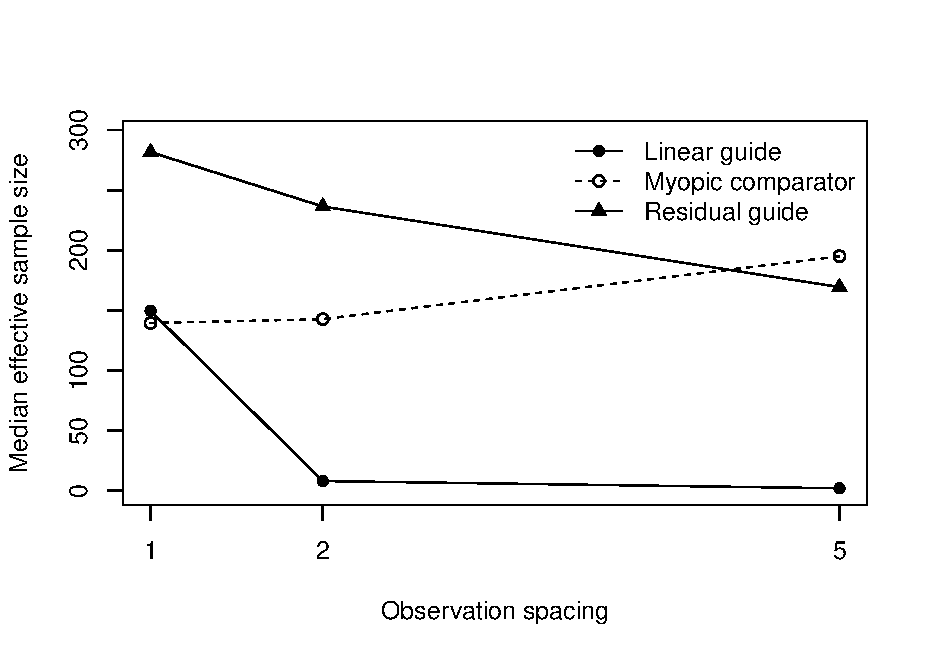
\includegraphics[width=0.72\textwidth]{figures/ess-against-spacing.pdf}
\caption{Effective sample size against observation spacing. Filled circles: linear guide, the medians in Table~\ref{tab:s1}. Open circles: myopic comparator, which is not the prediction. The myopic values are those stated in the text.}
\label{fig:ess}
\end{figure}

From Table~\ref{tab:s1}, the linear median effective sample size is 149.660679297905 at spacing 1 and 2.05670742297318 at spacing 5. The value at spacing 5 is smaller, so the prediction holds. At spacing 2 the linear median is 8.09166818813341. At every linear row, the median that includes zero weights equals the median computed on the finite weights alone. The fall is present in the finite weights. The median proportion of invalid draws is 0.0329 at spacing 1, 0.009 at spacing 2 and 0 at spacing 5, so the fall at spacing 5 is not produced by the zero-weight rule.

At spacing 1 the myopic median is 139.525563697813. At spacing 2 it is 142.824313796391. At spacing 5 it is 195.181391518181. The myopic median does not fall as the spacing grows.

Two qualifications belong with the comparison. The guide was given the simulated prevalence and the simulated contact-rate path. The result is about \(h^{*}\) given those paths. At spacing 1 the linear median is 149.660679297905 out of 500 draws, so the guide is already uneven on the published grid. The prediction was the comparison across spacings, not a claim that the published grid is unaffected. The comparison does not measure a pathwise distance to the true conditioned process, and it does not say whether a filtering distribution would change.

\section{Discussion}
\label{sec:discussion}

We have given a reading of the linear incidence guide in \citet{whitaker2025} and a diagnostic for its weights under coarser observation. The constant-hazard step is the linearity assumption named in their limitations section. On the printed importance weight, a poor conditioned hazard changes the proposal and the weights. We have shown, on the synthetic mechanism of their Section 4.1, that the median effective sample size of the linear guide is smaller at spacing 5 than at spacing 1, with the values in Table~\ref{tab:s1}. The myopic comparator does not fall. The guide had the simulated state and the simulated contact-rate path, and even the published spacing already yields a median well below the number of draws.

We expect the diagnostic to be useful when an observation window is lengthened and the question is whether this proposal is the source of uneven weights. We do not expect it to certify a posterior, and we do not treat it as a threshold that divides adequate spacing from inadequate spacing. The three spacings were chosen before the run because they divide the published horizon. They are not estimated change-points.

A replacement of \(q\) remains future work. Equation (19) of \citet{golightly2019} samples a Markov jump process with a linear-noise conditioned hazard, and the weight (3) is the jump-process likelihood ratio under a Gaussian observation of the state. Algorithm~\ref{alg:schematic} divides by the density of Poisson incidence increments on a fixed grid. Equation (19) does not provide that density. Theorem 4.2 of \citet{corstanje2023} gives the ratio (16) for an inhomogeneous Poisson process conditioned on an exact integer end-point, and (16) contains \(h(0, x_0)\). We do not drop that factor, and we do not place either construction in the denominator of Equation~\eqref{eq:weight}. Further work needs a proposal whose evaluated density is the density of the same incidence increments that the numerator describes.

The weekly Ebola series and the weekly COVID-19 series in \citet{whitaker2025} are not analysed. The counts are not stored in this repository, and we do not read them off the published figures. A surveillance example would need those counts in a form that can be reproduced, and a claim that the simulations have not already settled.


\section*{Acknowledgements}
This draft records a diagnostic study. No personal acknowledgements are attached.

\section*{Funding details}
Funding details have not been supplied for this draft.

\section*{Disclosure statement}
The authors report there are no competing interests to declare.

\section*{Data availability}
All data used in this paper were simulated from the model stated in Section~\ref{sec:simulation}. The table and the figure are regenerated by the script named in the supplementary note.

\section*{Supplementary material}
The supplement for this draft is the base R code that evaluates the linear guide and the residual guide, the two study scripts, the stored tables, and the reproduction script. No surveillance counts are included.

\bibliographystyle{plainnat}
\bibliography{references}

\end{document}
